\documentclass{article}
\usepackage[utf8]{inputenc}
\usepackage{amsthm}
\usepackage{amssymb}
\usepackage{amsmath}
\usepackage{amsfonts}
\usepackage{latexsym}
\usepackage{graphicx}
\usepackage{float}
\usepackage{listings}
\usepackage{xcolor}
\usepackage{imakeidx}
\usepackage{algpseudocode}
\usepackage{hyperref}
\usepackage{textcomp}
\usepackage{qrcode}
\graphicspath{ {../figures/} }

\newcommand{\N}{\mathbb{N}}
\newcommand{\Z}{\mathbb{Z}}
\newcommand{\E}{\mathbb{E}}
\newcommand{\R}{\mathbb{R}}
\newcommand{\LL}{\mathcal{L}}
\newcommand{\PP}{\mathcal{P}}
\newcommand{\HH}{\mathcal{H}}
\newcommand{\KK}{\mathcal{K}}
\newcommand{\XX}{\mathcal{X}}
\newcommand{\Zm}{\Z/m\Z}
\newcommand{\Zn}{\Z/n\Z}
\newcommand{\Zp}{\Z_p}
\newcommand{\Zmn}{\Z/mn\Z}
\newcommand{\s}{\vspace*{0.4 cm}}
\newcommand{\nd}{\noindent}
% \newcommand{\mactors}{\texttt{MIN\textunderscore ACTORS}}


\definecolor{codegreen}{rgb}{0,0.6,0}
\definecolor{codegray}{rgb}{0.5,0.5,0.5}
\definecolor{codepurple}{rgb}{0.58,0,0.82}
\definecolor{backcolour}{rgb}{255,255,255}

\lstdefinestyle{mystyle}{
    backgroundcolor=\color{backcolour},
    commentstyle=\color{codegreen},
    keywordstyle=\color{magenta},
    numberstyle=\tiny\color{codegray},
    stringstyle=\color{codepurple},
    basicstyle=\ttfamily\footnotesize,
    breakatwhitespace=false,
    breaklines=true,
    captionpos=b,
    keepspaces=true,
    numbers=left,
    numbersep=5pt,
    showspaces=false,
    showstringspaces=false,
    showtabs=false,
    tabsize=2
}
\lstset{style=mystyle}


\title{An exact and fast algorithm for computing top-k closeness centrality}
\author{Luca Lombardo}
\date{Univeristy of Pisa - Department of Mathematics}


\begin{document}
\maketitle

\begin{abstract}
    TO DO!
% Given a connected graph $G=(V,E)$, the closeness centrality of a vertex $v$ is defined as $ \frac{n-1}{\sum_{w \in V} d(v,w)}$. This measure is widely used in the analysis of real-world complex networks, and the problem of selecting the $k$ most central vertices has been deeply analysed in the last decade. However, this problem is computationally not easy, especially for large networks. I propose an algorithm for selecting the $k$ most central nodes in a graph: I experimentally show that this algorithm improves significantly both the textbook algorithm, which is based on computing the distance between all pairs of vertices, and the state of the art. Finally, as a case study, I compute the $10$ most central actors in the IMDB collaboration network, where two actors are linked if they played together in a movie.

% Da cambiare le parole, preso dal paper

\end{abstract}

\newpage
\tableofcontents{}
\section{Introduction}
A graph $G= (V,E)$ is a pair of a sets. Where $V = \{v_1,...,v_n\}$ is the set of \emph{nodes}, and $E \subseteq V \times V, ~ E = \{(v_i,v_j),...\}$  is the set of \emph{edges} (with $|E| = m \leq n^2$). \s

\nd In this paper we discuss the problem of identifying the most central nodes in a network using the measure of \emph{closeness centrality}. Given a connected graph, the closeness centrality of a node $v \in V$ is defined \cite{Sodeur2019} as the reciprocal of the sum of the length of the shortest paths between the node and all other nodes in the graph. Normalizing, we obtain the following formula:

\begin{equation}\label{closeness}
   c(v) = \frac{n-1}{\displaystyle \sum_{w \in V} d(v,w)}
\end{equation}

\nd where $n$ is the cardinality of $V$ and $d(v,w)$ is the distance between $v,w \in V$. This is a very powerful tool in the analysis of a network: it ranks each node telling us the most efficient ones in spreading information through all the other nodes in the graph. As mentioned before, the denominator of this definition give us the length of the shortest path between two nodes. This means that for a node to be central, the average number of links needed to reach another node has to be low. The goal of this paper is to computer the $k$ nodes with the higher closeness centrality. \s

\noindent As case study we will use the collaboration network in the \emph{Internet Movie Database} (IMDB).  We will consider two different graphs. For the first one we define an undirected graph $G=(V,E)$ where
\begin{itemize}
    \item The nodes $V$ are the actors and the actress
    \item The non oriented edges in $E$ links two nodes if they played together in a movie.
\end{itemize}
For the second one we will do the opposite thing. We define an undirected graph $G=(V,E)$ where:
\begin{itemize}
    \item the nodes $V$ are the movies.
    \item the non oriented edges in $E$ links two movies if they have an actor or actress in common.
\end{itemize}

\clearpage
\subsection{The Problem}

Since we are dealing with a web-scale network any brute force algorithm would require years to end. The main difficulty here is caused by the computation of distance $d(v,w)$ in \eqref{closeness}. This is a well know problem known as \emph{All Pairs Shortest Paths} (or \emph{APSP problem}). \s

\noindent We can solve the APSP problem either using the fast matrix multiplication or, as made in this paper, implementing a breath-first-search (BFS) method. There are several reason to prefer this second approach over the first one in this type of problems. \s

\noindent A graph is a data structure and we can describe it in different ways \cite{skienna08}. Choosing one over another can have an enormous impact on performance. In this case, we need to remember the type of graph that we are dealing with: a very big and sparse one. The fast matrix multiplication implement the graph as an $n\times n$ matrix where the position $(i,j)$ is zero if the nodes $i,j$ are not linked, 1 (or a specific number if weighted) otherwise. This method requires $O(n^2)$ space in memory. That is an enormous quantity on a web-scale graph. Furthermore the time complexity is $O(n^{2.373} \log n)\}$ \cite{10.1145/567112.567114}  \s

\noindent Using the BFS method the space complexity is $O(n+m)$, which is a very lower value compared to the previous method. In terms of time, the complexity is $O(nm)$. Unfortunately, this is not enough to compute all the distances in a reasonable time. It has also been proven that this method can not be improved. In this paper I propose an exact algorithm to compute efficiently only the top-$k$ nodes with the higher closeness centrality.

\section{The algorithm}

In a connected graph, given a node $v \in V$, we can define its farness as

\begin{equation}
    f(v) = \frac{1}{c(v)} = \frac{1}{n-1} \displaystyle \sum_{w \in V} d(v,w)
\end{equation}
where $c(v)$ is the closeness centrality defined in \eqref{closeness}. Since we are working with a disconnected graph, a natural generalization of this formula is

\begin{equation}\label{wrong-farness}
    f(v) = \frac{1}{c(v)} = \frac{1}{r(v)-1} \displaystyle \sum_{w \in V} d(v,w)
\end{equation}
where $r(v) = |R(v)|$ is the cardinality of the set of reachable nodes from $v$. To avoid any problem during the computation, this formula still needs to be modified. Let's assume that the node $v$ that we are considering has just one link at distance $1$ with another node $w$ with \emph{out-degree} 0. If we consider the formula \eqref{wrong-farness} we will get a false result: $v$ would appear to be very central, even if it's obviously very peripheral. To avoid this problem, we can generalize the formula \eqref{wrong-farness} normalizing as suggested in \texttt{[Lin 1976; Wasserman and Faust 1994; Boldi and Vigna 2013; 2014; Olsen et al. 2014]}

\begin{equation}\label{farness}
    f(v) = \frac{n-1}{(r(v)-1)^2} \sum_{w \in R(v)} d(v,w)
\end{equation}
With the convention that in a case of $\frac{0}{0}$ we set the closeness of $v$ to 0

\subsection{The lower bound technique}
During the computation of the farness, for each node, we have to compute the distance from that node and to all the other ones reachable from it. Since we are dealing with millions of nodes, it's not possibile in a reasonable time. In order to compute only the top-$k$ most central node we need to find a way to avoid computing BFS for nodes that won't be in the top-$k$. \s

\noindent The idea is to keep track of a lower bound on the farness for each node that we will compute. If the lower bound tell us that the node will not be in the top-$k$, this will allow us to kill the BFS operation before it reaches the end. More precisely:

\begin{itemize}
    \item The algorithm will compute the farness of the first $k$ nodes, saving them in a vector \texttt{top}. From now on, this vector will be full.

    \item Then, for all the next nodes, it defines a lower bound
    \begin{equation}\label{lower-bound}
        \frac{n-1}{(n-1)^2} (\sigma_{d-1} + n_d \cdot d)
    \end{equation}

    where $\sigma_d$ is the partial sum in \eqref{farness} at the level of exploration $d$. The lower bound \eqref{lower-bound} is updated every time that we change level of exploration during the BFS. In this way, if at a change of level the lower bound of the vertex that we are considering is bigger than the $k-th$ element of \texttt{top}, we can kill the BFS. The reason behind that is very simple: the vector \texttt{top} is populated with the top-k nodes in order and the farness is inversely proportional to the closeness centrality. So if at that level $d$ the lower bound is already bigger than the last element of the vector, there is no need to compute the other level of the BFS since it will not be added in \texttt{top} anyway. \s

    The \eqref{lower-bound} it's a worst case scenario, and that makes it perfect for a lower bound. If we are at the level $d$ of exploration, we have already computed the sum in \eqref{farness} up to the level $d-1$. Then we need to consider in our computation of the sum the current level of exploration: the worst case gives us that it's linked to all the nodes at distance $d$. We also put $r(v)=n$, in the case that our graph is strongly connected and all nodes are reachable form $v$.
\end{itemize}

\textsc{Scrivere pseudocodice}


% \begin{algorithmic}[H] \caption{How to write algorithms}
%     \KwIn{A graph $G = (V,E)$}
%     \KwOut{Top-$k$ nodes with higher closeness centrality and their value} \
%     \

%     \While{not at end of this document}{
%      read current\;
%      \eIf{understand}{
%       go to next section\;
%       current section becomes this one\;
%       }{
%       go back to the beginning of current section\;
%      }
%     }

%    \end{algorithmic}

\section{The IMDB Case Study}
The algorithm shown before can be applied to any dataset on which is possibile to build a graph on. In this case we are considering tha data taken from the \emph{Internet Movie Database} (IMDB).

\subsection{Data Structure}
All the data used can be downloaded here: \url{https://datasets.imdbws.com/} \s

\noindent In particolar we're interest in 3 files
\begin{itemize}
    \item \texttt{title.basics.tsv}
    \item \texttt{title.principals.tsv}
    \item \texttt{name.basics.tsv}
    \item \texttt{title.ratings.tsv}
\end{itemize}
Let's have a closer look to this 4 files:

\subsubsection*{title.basics.tsv}
\emph{Contains the following information for titles:}
\begin{itemize}
    \item \texttt{tconst} (string) - alphanumeric unique identifier of the title
    \item \texttt{titleType} (string) – the type/format of the title (e.g. movie, short, tvseries, tvepisode, video, etc)
    \item \texttt{primaryTitle} (string) – the more popular title / the title used by the filmmakers on promotional materials at the point of release
    \item \texttt{originalTitle} (string) - original title, in the original language
    \item \texttt{isAdult} (boolean) - 0: non-adult title; 1: adult title
    \item \texttt{startYear} (YYYY) – represents the release year of a title. In the case of TV Series, it is the series start year
    \item \texttt{endYear} (YYYY) – TV Series end year.
    \item \texttt{runtimeMinutes} – primary runtime of the title, in minutes
    \item \texttt{genres} (string array) – includes up to three genres associated with the title
\end{itemize}

\subsubsection*{title.principals.tsv}
\emph{Contains the principal cast/crew for titles:}
\begin{itemize}
    \item \texttt{tconst} (string) - alphanumeric unique identifier of the title
    \item \texttt{ordering} (integer) – a number to uniquely identify rows for a given titleId
    \item \texttt{nconst} (string) - alphanumeric unique identifier of the name/person
    \item \texttt{category} (string) - the category of job that person was in
    \item \texttt{job} (string) - the specific job title if applicable
    \item \texttt{characters} (string) - the name of the character played if applicable
\end{itemize}

\subsubsection*{name.basics.tsv}
\emph{Contains the following information for names:}
\begin{itemize}
    \item \texttt{nconst} (string) - alphanumeric unique identifier of the name/person
    \item \texttt{primaryName} (string)– name by which the person is most often credited
    \item \texttt{birthYear} – in YYYY format
    \item \texttt{deathYear} – in YYYY format if applicable
    \item \texttt{primaryProfession} (array of strings)– the top-3 professions of the person
    \item \texttt{knownForTitles} (array of tconsts) – titles the person is known for
\end{itemize}

\subsubsection*{title.ratings.tsv}
\emph{Contains the following information for titles:}
\begin{itemize}
    \item \texttt{tconst} (string) - alphanumeric unique identifier of the title
    \item \texttt{averageRating} – weighted average of all the individual user ratings
    \item \texttt{numVotes} – number of votes the title has received
\end{itemize}

\newpage
\subsection{Filtering} \label{filtering}

This is a crucial section for the algorithm in this particolar case study. This raw data contains a huge amount of un-useful information that will just have a negative impact on the performance during the computation. We are going to see in detail all the modification made for each file. All this operation have been implemented using \texttt{python} and the \texttt{pandas} library. \s

\nd Since we want to build two different graph, some consideration will have to be made for the specific case. If nothing is told it means that the filtering of that file is the same for both graphs.

\subsubsection{name.basics.tsv}

For this file we only need the following columns

\begin{itemize}
    \item \texttt{nconst}
    \item \texttt{primaryTitle}
    \item \texttt{primaryProfession}
\end{itemize}
Since all the actors starts with the string \texttt{nm0} we can remove it to clean the output. Furthermore a lot of actors/actresses do more than one job (director etc..). To avoid excluding important actors we consider all the ones that have the string \texttt{actor/actress} in their profession. In this way, both someone who is classified as \texttt{actor} or as \texttt{actor, director} is taken into consideration. \s

\noindent Then we can generate the final filtered file \texttt{Attori.txt} that has only two columns: \texttt{nconst} and \texttt{primaryName}


\subsubsection{title.basics.tsv}

For this file we only need the following columns

\begin{itemize}
    \item \texttt{tconst}
    \item \texttt{primaryTitle}
    \item \texttt{isAdult}
    \item \texttt{titleType}
\end{itemize}
Since all the movies starts with the string \texttt{t0} we can remove it to clean the output. In this case, we also want to remove all the movies for adults. This part can be optional if we are interest only in the closeness and harmonic centrality. Even if the actors and actresses of the adult industry use to make a lot of movies together, this won't alter the centrality result. As we know, an higher closeness centrality can be seen as the ability of a node to spread efficiently information in the network. Including the adult industry would lead to the creation of a very dense and isolated neighborhood. But none of those nodes will have an higher closeness centrality because they only spread information in their community. This phenomenon will be discussed more deeply in the analysis of the graph visualized. \s

\noindent We can also notice that there is a lot of \emph{junk} in IMDb. To avoid dealing with un-useful data, we are considering all the non-adult movies in this whitelist

\begin{itemize}
    \item \texttt{movie}
    \item \texttt{tvSeries}
    \item \texttt{tvMovie}
    \item \texttt{tvMiniSeries}
\end{itemize}
The reason to only consider this categories is purely to optimize the performance during the computation. On IMDb each episode is listed as a single element: to remove them without loosing the most important relations, we only consider the category \texttt{tvSeries}. This category lists a TV-Series as a single element, not divided in multiple episodes. In this way we will loose some of the relations with minor actors that may appear in just a few episodes. But we will have preserved the relations between the protagonists of the show. \s

\noindent Then we can generate the final filtered file \texttt{FilmFiltrati.txt} that has only two columns: \texttt{tconst} and \texttt{primaryTitle}

\subsubsection{title.principals.tsv}

This file is needed for the analysis of both graphs, but there some different observation between them. For the both we only need the following columns

\begin{itemize}
    \item \texttt{tconst}
    \item \texttt{nconst}
    \item \texttt{category}
\end{itemize}

\noindent As before, we clean the output removing unnecessary strings. \s

\textsc{Actors Graph}
\s

\noindent Using the data obtained  before we create an array of unique actor ids (\texttt{nconst}) and an array of how may times they appear (\texttt{counts}). This will give us the number of movies they appear in. And here it comes the core of the optimization for this graph. Let's define a constant \texttt{MINMOVIES}. This integer is the minimum number of movies that an actor needs to have made in his carrier to be considered in this graph. The reason to do that it's purely computational. If an actor/actress has less then a reasonable number of movies made in his carrier, there is an high probability that he/she has an important role in our graph during the computation of the centralities. \s

\textsc{Movies Graph} \s

\noindent For this graph we don't need any optimization on this file. We just clean clean the output and leave the rest as it is. \s

\nd At the end, for both graph, we can finally generate the file \texttt{Relazioni.txt} containing the columns \texttt{tconst} and \texttt{nconst}

\subsubsection{title.ratings.tsv}

This file is necessary just in the analysis of the movie graph, it won't be even downloaded for the analysis of the actors graph. We will only need the following columns

\begin{itemize}
    \item \texttt{tconst}
    \item \texttt{numVotes}
\end{itemize}

\nd The idea behind the optimization made in this file is the same that we have used before with the \texttt{MINMOVIES} technique. We want to avoid computing movies that are not central with an high probability. To do that we consider the number of votes that each movie has received on the IMDB website. To do that we introduce the constant \texttt{VOTES}, considering only the movies with an higher number of votes. During the analysis we will change this value to see how it effects the list of the top-k most central movies. \s

\nd In this case we don't have to generate a new file, we can apply this condition to \texttt{FilmFiltrati.txt}

\section{An overview of the code}
The algorithm implement is multi-threaded and written in C\texttt{++}. To avoid redundances, we'll take in exame only the \emph{Actors Graph} case.

\subsection{Data structures}
In this case we are working with two simple \texttt{struct} for the classes \emph{Film} and \emph{Actor}

\lstinputlisting[language=c++]{code/struct.cpp}
\s
\nd Then we need two dictionaries build like this

\lstinputlisting[language=c++]{code/map.cpp}
\s
\nd We are considering the files \texttt{Attori.txt} and \texttt{FilmFiltrati.txt}, we don't need the relations one for now. Once that we have read this two files, we loop on each one brutally filling the two dictionaries created before. If a line is empty, we skip it. We are using a try and catch approach. Even if the good practice is to use it only for a specific error, since we are outputting everything on the terminal it makes sense to \emph{catch} any error.

\lstinputlisting[language=c++]{code/data.cpp}
\s

Now we can use the file \texttt{Relazioni.txt}. As before, we loop on all the elements of this file, creating the variables

\begin{itemize}
    \item \texttt{id\textunderscore film}: index key of each movie
    \item \texttt{id\textunderscore attore}: index key of each actor
\end{itemize}

\nd If they both exists, we update the list of indices of movies that the actor/actresses played in. In the same way, we update the list of indices of actors/actresses that played in the movies with that id.

\lstinputlisting[language=c++]{code/graph.cpp}
\s
Now that we have defined how to build this graph, we have to implement the algorithm what will return the top-k central elements. \s

\nd The code can be found here: \url{https://github.com/lukefleed/imdb-graph}
\s
\begin{center}
    \qrcode{https://github.com/lukefleed/imdb-graph}
\end{center}

\subsection{Results - Actors Graph}

Here are the top-10 actors for closeness centrality obtained with the variable \texttt{MIN\textunderscore ACTORS=5} (as we'll see in the next section, it's the most accurate)

\begin{table}[h!]
    \centering
     \begin{tabular}{||c c||}
     \hline
     Node & Closeness centrality \\ [0.5ex]
     \hline\hline
     Eric Roberts & 0.324895 \\
     Christopher Lee &0.319873 \\
     Franco Nero & 0.31946 \\
     John Savage & 0.316258 \\
     Michael Madsen & 0.314451 \\
     Udo Kier & 0.31357 \\
     Geraldine Chaplin & 0.313141 \\
     Malcolm McDowell & 0.313014 \\
     David Carradine & 0.312648 \\
     Christopher Plummer & 0.311859 \\ [1ex]
     \hline
     \end{tabular}
\end{table}

\nd All the other results are available in the Github repository for all the values of \texttt{MIN\textunderscore ACTORS} and for $k=100$

\newpage
\subsection{Results - Movies Graph}

Here are the top-10 movies for closeness centrality obtained with the variable \texttt{VOTES=500} (as we'll see in the next section, it's the most accurate)

\begin{table}[h!]
    \centering
     \begin{tabular}{||c c||}
     \hline
     Node & Closeness centrality \\ [0.5ex]
     \hline\hline
     Merlin & 0.290731 \\
     The Odyssey & 0.290314 \\
     The Color of Magic	& 0.285208 \\
     The Godfather Saga	& 0.284932 \\
     Jack and the Beanstalk: The Real Story & 0.283522 \\
     In the Beginning & 0.28347 \\
     RED 2 & 0.283362 \\
     Lonesome Dove & 0.283353 \\
     Moses & 0.282953 \\
     Species & 0.282642 \\ [1ex]
     \hline
     \end{tabular}
\end{table}

\nd All the other results are available in the Github repository for all the values of \texttt{VOTES} and for $k=100$

\section{Analysis of the results}
In this section we are going to discuss the results of the top-k algorithm applied to the IMDb graphs. We are particularly interested in two factors:
\begin{itemize}
    \item The time needed to for the execution in function of different filtering values.
    \item The discrepancy on the results while varying the filtering values
\end{itemize}
The first one will tell us how much more efficient the algorithm is in terms of time, independently from the results. The second one is the metric to understand how accurate the filtered algorithm is. It's clear that even if we can compute the algorithm 100 times faster, it's of no use if the results are completely different from the real ones.\s

\nd The platform for the tests is \emph{a laptop}, so can not be considered precise due factors as thermal throttling. The CPU is an Intel(R) Core™ i7-8750H (6 cores, 12 threads), equipped with 16GB of DDR4 @2666 MHz RAM.

\subsection{Actors graph} \label{actors-graph}
Let's take into analysis the graph were each actors is a node and two nodes are linked the if they played in a movie together. In the case, during the filtering, we created the variable \texttt{MIN\textunderscore ACTORS}. This variable is the minimun number of movies that an actor/actress has to have done to be considered in the computation.

Varying this variable obviously affects the algorithm, in different way. The higher this variable is, the less actors we are taking into consideration. So, with a smaller graph, we are expecting better results in terms of time execution. On the other hand, we also can expect to have less accurate results. What we are going to discuss is how much changing \texttt{MIN\textunderscore ACTORS} affects this two factors

\subsubsection{Time of execution}

TO DO

\subsubsection{Discrepancy of the results}
We want to analyze how truthful our results are while varying \texttt{MIN\textunderscore ACTORS}. The methodology is simple: for each results (lists) we take the intersection of the two. This will return the number of elements in common. Knowing the length of the lists, we can find the number of elements not in common. \s

\nd A way to see this results is with a square matrix $n \times n, ~ A = (a_{ij})$, where $n$ is the number of different values that we gave to \texttt{MIN\textunderscore ACTORS} during the testing. In this way the $(i,j)$ position is the percentage of discrepancy between the results with \texttt{MIN\textunderscore ACTORS} set as $i$ and $j$ \s

\nd This analysis is implemented in python using the \texttt{pandas} and \texttt{numpy} libraries.

\lstinputlisting[language=c++]{code/closeness_analysis.py}

\nd Visualizing this analysis we obtain this

\begin{figure}[h] \label{matrix-a}
    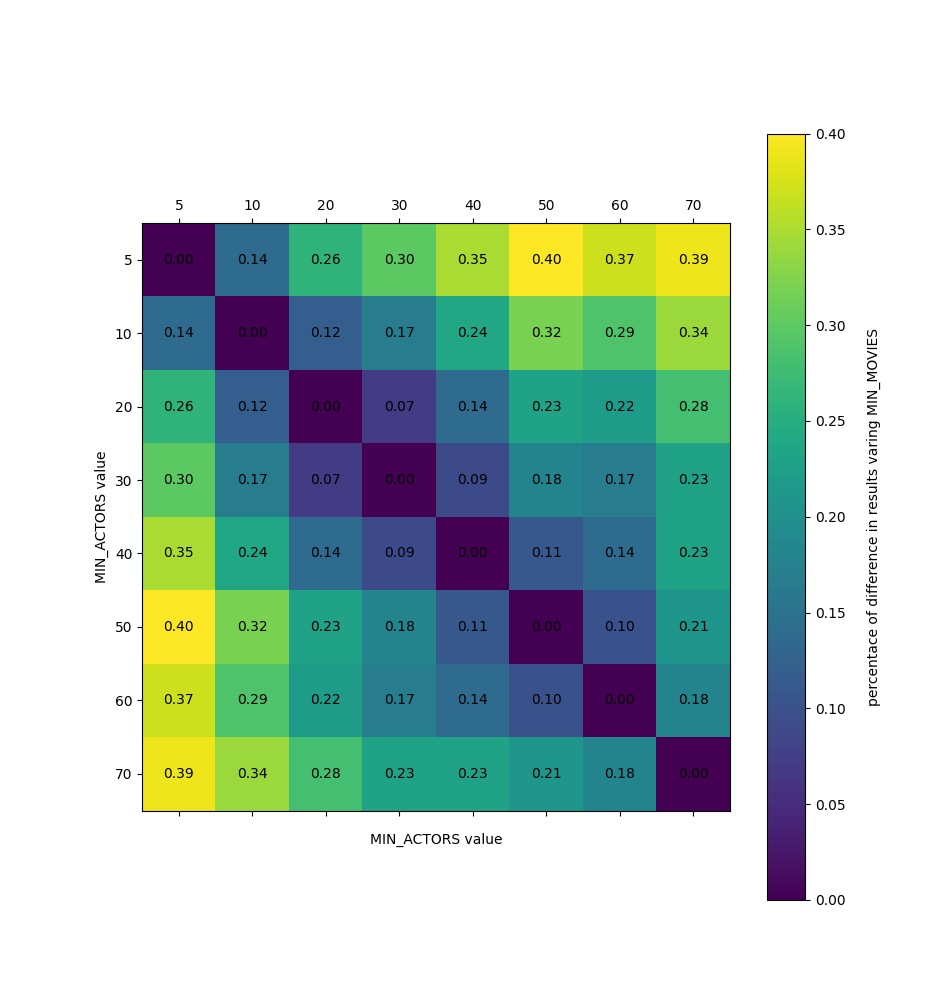
\includegraphics[width=12cm]{Figure_1.png}
    \caption{Discrepancy of the results on the actors graph in function of the minimum number of movies required to be considered as a node}
\end{figure}

\nd As expected, the matrix is symmetrical and the elements on the diagonal are all equal to zero. We can see clearly that with a lower value of \texttt{MIN\textunderscore ACTORS} the results are more precise. The discrepancy with \texttt{MIN\textunderscore ACTORS=10} is 14\% while being 39\% when \texttt{MIN\textunderscore ACTORS=70}. \s

\nd This is what we obtain confronting the top-k results when $k=100$. It's interesting to se how much the discrepancy change with different values of $k$. However, choosing a lower value for $k$ would not be useful for this type of analysis. Since we are looking at the not common elements of two lists, with a small length, we would get results biased by statistical straggling. \s

\textsc{Da fare: test con con k=500 e k=1000}

\s
\newpage
\subsection{Movies Graphs}
In this section we are taking into consideration the graph build over the movies and their common actors/actresses. Due to an elevated number of nodes, to optimize the performance during the execution in the section \ref{filtering} we introduced the variable \texttt{VOTES}. It represents the minimum number of votes (indifferently is positive or negative) that a movie need to have on the IMDb database to be considered as a node in our graph.

As seen during the analysis of the actors graph in \ref{actors-graph}, varying this kind of variables affects the results in many ways. All the observations made before are still valid for this case, I won't repeat them for shortness. As done before (\ref{matrix-a}), we are going to use a matrix to visualize and analyze the results
\s

% \lstinputlisting[language=c++]{code/closeness_analysis_2.py}

\nd Giving us:
\begin{figure}[H] \label{matrix-b}
    \centering
    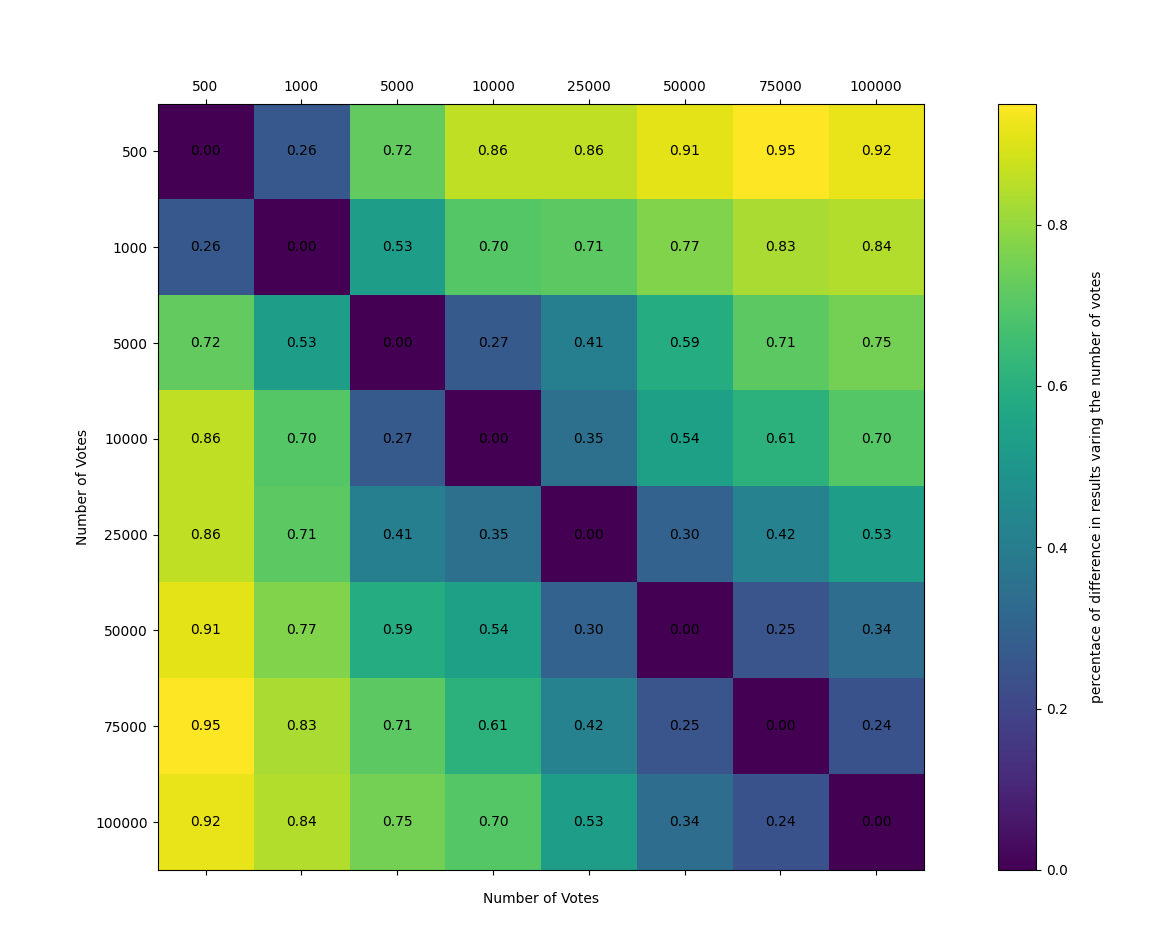
\includegraphics[width=13cm]{Figure_2.png}
    \caption{Discrepancy of the results on the movie graph in function of the minimum number of votes required to be considered as a node}
\end{figure}
\newpage
\lstinputlisting[language=c++]{code/closeness_analysis_2.py}

\s \nd \emph{Dire qualcosa sull'analisi, ma andrebbe rifatta perché i valori non vanno bene}

\section{Visualization of the graphs}
Graphs are fascinating structures, visualizing them can give us a more deep understanding of their proprieties. Since we are dealing with millions of nodes, displaying them all would be impossibile, especially on a web page. \s

\nd For each case we need to find a small (in the order of 1000) subset of nodes $S \subset V$ that we want to display. It's important to take into consideration, as far as we can, nodes that are "important" in the graph \s

\nd All this section is implemented in python using the library \texttt{pyvis}. The goal of this library is to build a python based approach to constructing and visualizing network graphs in the same space. A pyvis network can be customized on a per node or per edge basis. Nodes can be given colors, sizes, labels, and other metadata. Each graph can be interacted with, allowing the dragging, hovering, and selection of nodes and edges. Each graph's layout algorithm can be tweaked as well to allow experimentation with rendering of larger graphs. It is designed as a wrapper around the popular Javascript \texttt{visJS} library

\subsection{Actors Graph} \label{actors-graph-vis}
For the actors graph, we take the subset $S$ as the actors and actresses with at least 100 movies made in their carrier. We can immediately deduct that this subset will be characterized by actors and actresses of a certain age. It takes time to make 100 movies. But as we have seen, having an high number of movies made, it's a good estimator for the closeness centrality. It's important to keep in mind that the graph will only show the relations within this subset. This means that even if an actor has 100 movies made in his carrier, in this graph the relative node may have just a few relations. We can see this graph as a collaboration network only between the most popular actors and actresses. \s

\nd An interactive version can be found at this web page. It will take a few seconds to render, it's better to use a computer and not a smartphone. \s

\textsc{Interactive version}: \url{https://lukefleed.xyz/imdb-graph.html}

\begin{center}
    \s \nd \qrcode{https://lukefleed.xyz/imdb-graph.html}
\end{center}

\begin{figure}[H] \label{imdb-a-network}
    \centering
    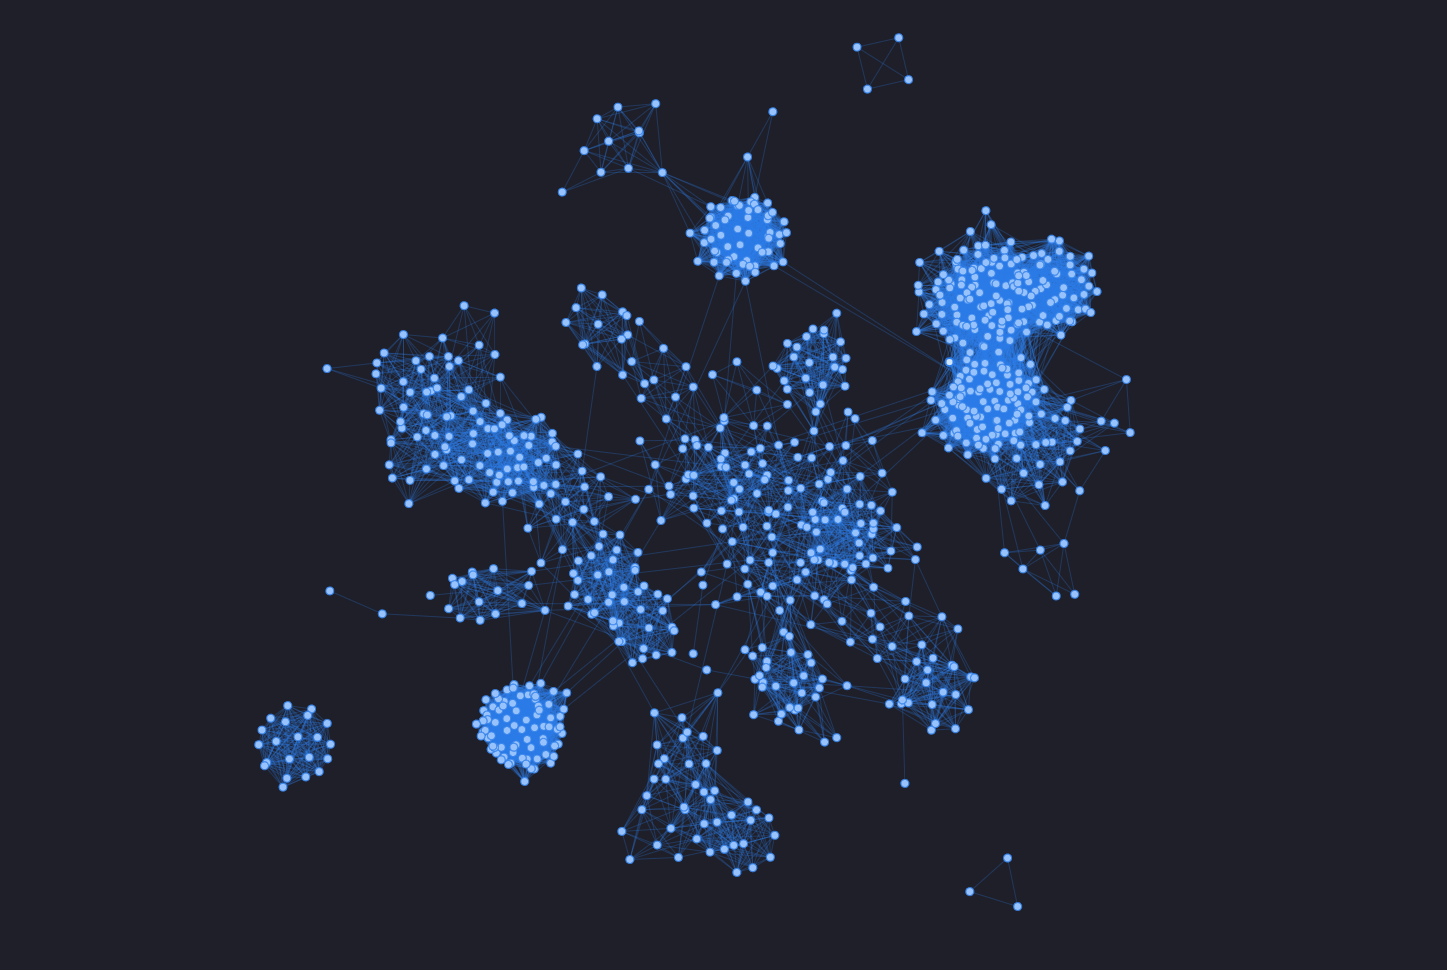
\includegraphics[width=13cm]{Screenshot.png}
    \caption{\emph{The collaboration network of the actors and actresses with more that an 100 movies on the IMDb network}}
\end{figure}

The result obtained is extremely interesting. We can clearly see how this graph it's characterized by different (and some times isolated) communities. The nodes in them are all actors and actresses of the same nationality. There are some very big clusters as the \emph{Bollywood}'s one that are almost isolated. Due to cultural and linguistic differences those actors never collaborated with anyone outside their country. \s

A visual analysis of this graph can reflects some of the proprieties that we saw during the analysis of the results. Let's take the biggest cluster, the Bollywood one. Even if it's very dense and the nodes have a lot of links, none of them ever appeared in out top-k results during the testing. This happens due to the proprieties of closeness centrality, the one that we are taking into consideration. It can be seen as the ability of a node to transport information efficiently into the graph. But the Bollywood's nodes are efficient in transporting information only in their communities since they don't collaborate with nodes of other clusters. \s

A simple and heuristic way to see this phenomena is by selecting in the interactive graph a node with an higher centrality and dragging him around. It will move and influence almost every community. If we repeat the same action with a Bollywood node, it will only move the nodes of his community, leaving almost un-moved all the other nodes.

\subsection{Movies Graph}

The methodology used for this graph is basically the same of \ref{actors-graph-vis}, however the results are slightly different. \s

\textsc{Interactive version}: \url{https://lukefleed.xyz/imdb-movie-graph.html}
\begin{center}
    \s \nd \qrcode{https://lukefleed.xyz/imdb-movie-graph.html}
\end{center}

\s

\begin{figure}[H] \label{imdb-m-network}
    \centering
    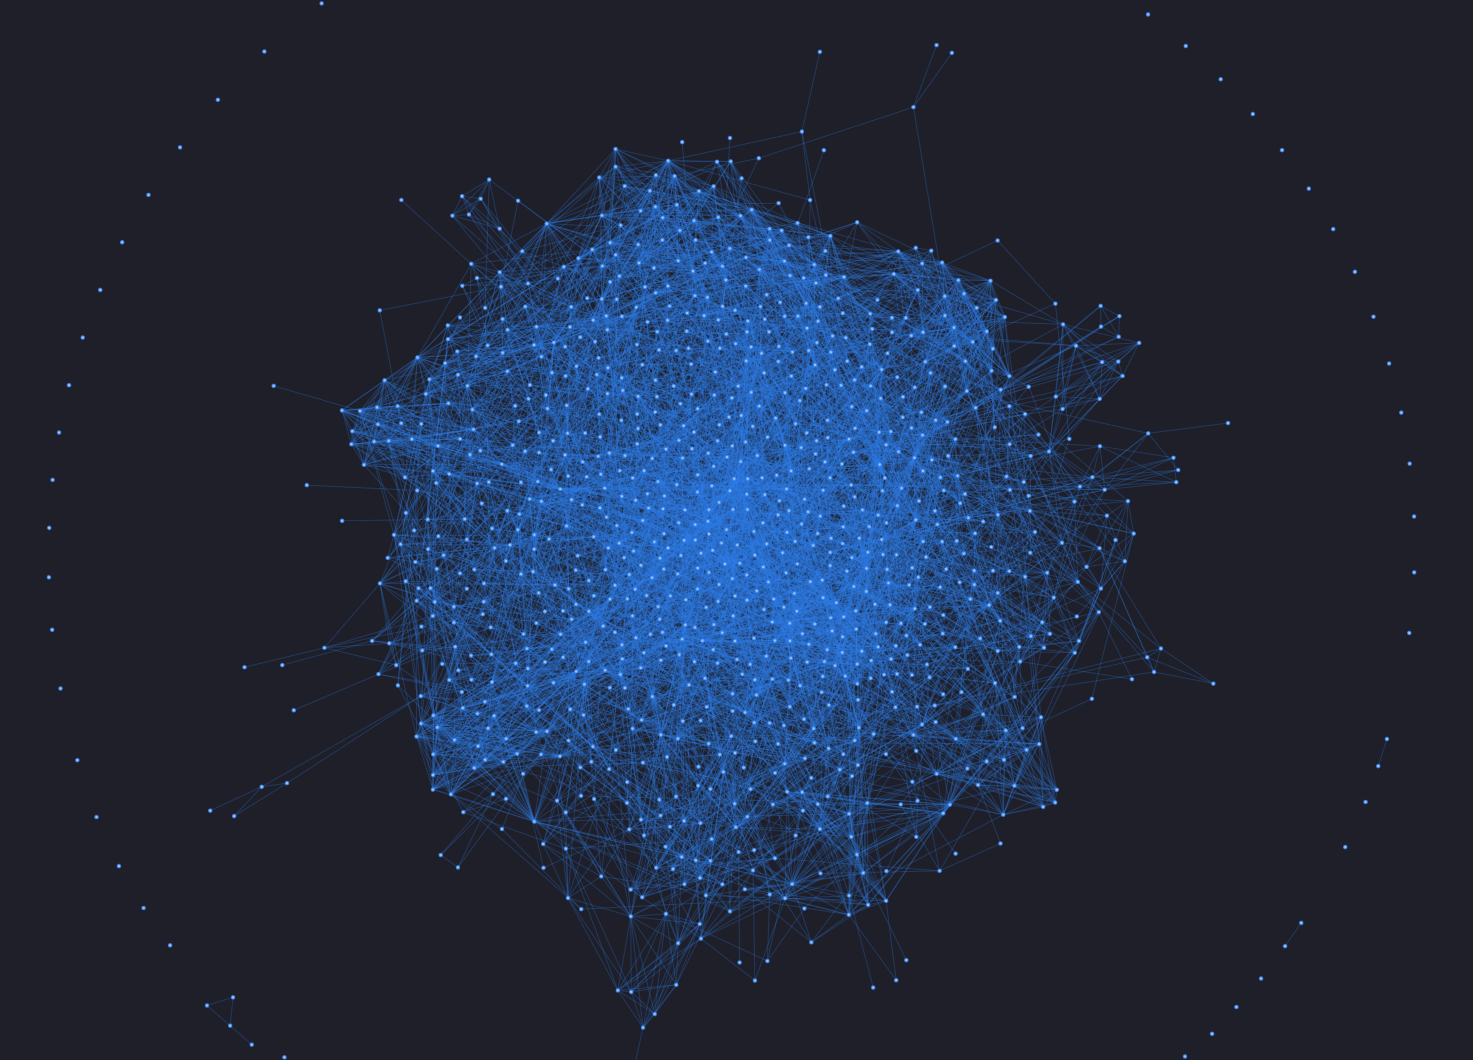
\includegraphics[width=13cm]{movie-graph.png}
    \caption{\emph{The network of the movies with more that an 500 votes on the IMDb database}}
\end{figure}

Even if at a first sight it may seem completely different from the previous one, it is not. As we can see, there are no evident communities. But some areas are more dense than other. If we zoom in in one of those areas we can see that the movies are often related. If there is a saga of popular movies, they will be very close in this graph. It's easy to find some big neighborhoods as the MCU (Marvel Cinematic Universe) one. \s

\nd Since we are considering about the top thousand most popular nodes, those movies are mostly from the Hollywood scene. So it makes sense that there are not isolated clusters.


\end{document}
